\documentclass[11pt,twocolumn]{article}
\usepackage{authblk}
\usepackage{pslatex, graphicx, amssymb, amsmath}
\usepackage{tikz}
\usepackage[hidelinks]{hyperref}
%%%% Redefine abstract environment
\def\abstract{
\typeout{Abstract}
 {\bf Abstract} 
} \def\endabstract{\par}


\begin{document}
\title{Solving the Carcassonne board game using reinforcement learning agents}
\author[1]{Bartosz Strzelecki}
\author[1]{Bogna Lew}
\author[1]{Jakub Kuczys}
\author[1]{Jakub Wierzba}
\author[1]{Krzysztof Pisarski}
\author[2]{Piotr Mironowicz}
\affil[1]{Faculty of Electronics, Telecommunications and Informatics, Gdańsk University of Technology, 80-233 Gdańsk, Poland}
\affil[2]{Department of Algorithms and System Modelling, Faculty of Electronics, Telecommunications and Informatics, Gdańsk University of Technology, 80-233 Gdańsk, Poland}


\maketitle
\begin{abstract}

  This article explores the use of artificial intelligence in board games, focusing
on the advancements from AlphaGo\cite{AlphaGoAlgorithm} and AlphaGo Zero\cite{AlphaGoZero}. 
AlphaGo marked a milestone in AI by defeating professional Go players using a 
combination of supervised learning and neural networks for policy and value estimation. 
AlphaGo Zero simplified the architecture by integrating policy and value evaluation 
into a single residual neural network and learning solely through self-play, 
eliminating reliance on human game data. Inspired by this approach, the development 
of a Carcassonne AI agent utilized a custom-built game engine designed for 
high computational efficiency and concurrency. The agent employs Monte Carlo Tree Search (MCTS) 
to navigate the game’s high branching factor and integrates policy and value-based 
evaluations for decision-making. Baseline strategies, such as greedy and random tactics, 
were implemented for performance comparison. The system design includes training 
environments and visualization tools, enabling detailed analysis of gameplay. 
This work lays a foundation for the development of an agent capable of professional play.
\small
\textbf{\textit{Keywords:}} machine learning, reinforced learning

  
\end{abstract}

\section{Introduction}
\label{chap:introduction}

In 2016 the world heard about a computer program named AlphaGo that in October 2015
won five to zero with Fan Hui, a Go professional and three-time European Champion. Later,
in March 2016 that same AI system won four to one with Lee Sedol, widely considered the
greatest player of that decade. Those revelations were groundbreaking considering that Go
was regarded as a major challenge for artificial intelligence. And yet AlphaGo managed not
only to master this game but also to devise innovative moves unknown to humans before \cite{AlphaGoBlog}.

Since then, we have noticed rapid development in this area. A crucial milestone was
the creation of AlphaGo Zero which, in contrast to its predecessors, used only reinforcement
learning during training and yet managed to outperform all the older versions in only forty
days \cite{AlphaGoZeroBlog}. Moreover, while the original AlphaGo algorithm used a complex setup
of four different neural networks for its decision-making, and required historical human games
for the training process, the AlphaGo Zero algorithm used only a single residual neural network,
and learned solely by self-play. Furthermore, the input size of AlphaGo Zero was also significantly
reduced by eliminating all hand-crafted features and leaving only the essential elements,
thus eliminating the need for any external knowledge during the learning process.

The next major milestone was the creation of AlphaZero. While this algorithm was largely similar
to its predecessor, it included modifications that allowed the generalisation to other games besides Go,
such as allowing for non-binary game outcomes and discontinuing the use of board rotations as a form of
data augmentation. That opened up opportunities for AI to master other games like Chess or Shogi.

As a result, the question arises whether it is possible to create an artificial intelligence
agent that can repeat AlphaGo and AlphaGo Zero's success in the area of more complex
board games like \textit{Settlers of Catan}, \textit{Pandemic}, \textit{Azul}, etc. This 
project attempts to answer this question by preparing an agent for the \textit{Carcassonne} game 
using reinforcement learning and analysing its behaviour and ability to make optimal 
decisions in a dynamic environment.

The following sections present the achieved goals. The section `Game engine architecture' 
presents the architecture of the game engine, its components and communication within the entire system. `Agent architecture' 
concentrates on describing the structure of the game agent and neural network input and
output structure. Next, the section `Evaluation' describes a design of the conducted experiment 
and the analysis of the agent's performance and its strategies.


\section{Game engine architecture}
New sections should not start with directly a subsection, rather with short section introduction. 

\subsection{Overview of architecture}
% Opisanie architektury silnika, sposobu komunikacji między komponentami, a także za co one odpowiadają.
Lorem ipsum dolor sit amet, consectetur adipiscing elit. Nam consectetur dignissim urna, a rhoncus dolor venenatis adipiscing. Phasellus viverra aliquam fringilla. Praesent mattis diam id ipsum placerat a laoreet diam tempus. Quisque eu leo ut sapien ultricies gravida ac sed turpis. Donec nibh enim, pretium a sagittis et, varius non nulla. Vivamus enim augue, condimentum eget convallis hendrerit, mattis ut lectus. Cum sociis natoque penatibus et magnis dis parturient montes, nascetur ridiculus mus. Proin semper libero augue. Praesent auctor ligula sit amet quam molestie adipiscing. Mauris vehicula congue mollis. Duis tincidunt interdum purus quis congue. Integer vel orci mauris. Curabitur rutrum tincidunt mi ut elementum. Nunc non massa nunc. Donec ultricies ipsum ac risus sollicitudin porta. Phasellus elementum odio et leo consectetur consectetur. 

Lorem ipsum dolor sit amet, consectetur adipiscing elit. Nam consectetur dignissim urna, a rhoncus dolor venenatis adipiscing. Phasellus viverra aliquam fringilla. Praesent mattis diam id ipsum placerat a laoreet diam tempus. Quisque eu leo ut sapien ultricies gravida ac sed turpis. Donec nibh enim, pretium a sagittis et, varius non nulla. Vivamus enim augue, condimentum eget convallis hendrerit, mattis ut lectus. Cum sociis natoque penatibus et magnis dis parturient montes, nascetur ridiculus mus. Proin semper libero augue. Praesent auctor ligula sit amet quam molestie adipiscing. Mauris vehicula congue mollis. Duis tincidunt interdum purus quis congue. Integer vel orci mauris. Curabitur rutrum tincidunt mi ut elementum. Nunc non massa nunc. Donec ultricies ipsum ac risus sollicitudin porta. Phasellus elementum odio et leo consectetur consectetur. 

\subsection{Components of a solution}
% Opisanie elementów z jakich się składa rozgrywka m.in.: kafelki i ich elementy, gracze, a także uwzględnione rozszerzenia gry Carcassonne.

The game Carcassone is played by placing tiles \cite{CarcassoneRules}. Each tile is represented by a set of features on it. All features are defined by their type, such as road, city, field or monastery, a modifier that modifies the calculation process, and the sides which indicate on which edges the feature is present. In this project there is only one modifier used - the shield. The engine was designed to accommodate game extensions. 

A feature's side is a byte sized value, in which each bit defines whether the feature is present on a specific half of the tile's edge as shown on Figure \ref{fig:SIDES}. Features such as roads, are represented by a whole edge formed by combining two sides e.g., the TopLeft and TopRight sides.
\begin{figure}
    \centering
    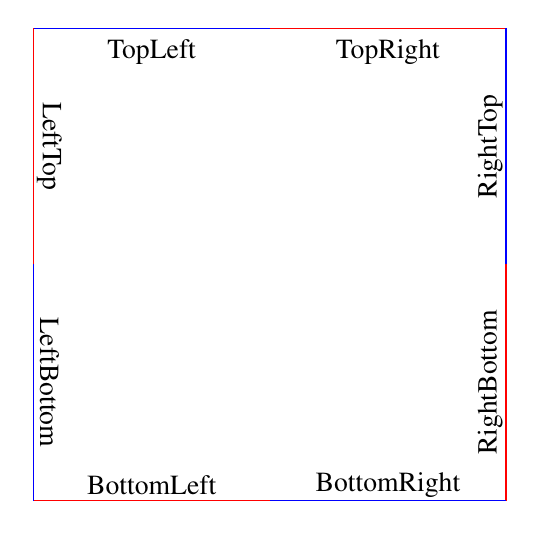
\begin{tikzpicture}
        %top line
        \draw [blue] (-3,3) -- (0,3);
        \draw [red] (0,3) -- (3,3);
        %right line
        \draw [blue] (3,3) -- (3,0);
        \draw [red] (3,0) -- (3,-3);
        %bottom line
        \draw [blue] (3,-3) -- (0,-3);
        \draw [red] (0,-3) -- (-3,-3);
        %left line
        \draw [blue] (-3,-3) -- (-3,0);
        \draw [red] (-3,0) -- (-3,3);
        
        \node at (-1.5, 2.7) {TopLeft};
        \node at (1.5, 2.7) {TopRight};
        
        \node [rotate=90] at (2.8, 1.5) {RightTop};
        \node [rotate=90] at (2.8, -1.5) {RightBottom};
        
        \node at (-1.5, -2.8) {BottomLeft};
        \node at (1.5, -2.8) {BottomRight};
        
	% czy może obrót 90stopni?
        \node [rotate=270] at (-2.8, 1.5) {LeftTop};
        \node [rotate=270] at (-2.8, -1.5) {LeftBottom};
    \end{tikzpicture}
    \caption{Side representation} \label{fig:SIDES}
\end{figure}

The tiles described do not contain information about their position or meeple placement. This information is located in the PlacedTile struct. The board is represented as a slice of placed tiles ordered by their placement, moreover it contains the used tile set, for verification whether the tile a player wants to place is legal. Additionally, board includes a city manager used for merging cities, scoring and checking for legal meeples placement in the cities.

A single game is represented by a board, shuffled deck of tiles, and players taking their turns. Each player knows their score, and the number of meeples of each type available to them.

Our solution has been designed to be modifiable by adding extensions to the game. Generalizations, such as meeple type or feature type, allow for the easy implementation of new potential features e.g., rivers.

\subsection{Execution flow}
% Opisanie wykonywanych akcji podejmowanych przez silnik gry: wylosowanie kafelka ze stosu, wyliczenie legalnych ułożeń kafelka, wybór położenia i wyliczanie punktacji za jego położenie.
Lorem ipsum dolor sit amet, consectetur adipiscing elit. Nam consectetur dignissim urna, a rhoncus dolor venenatis adipiscing. Phasellus viverra aliquam fringilla. Praesent mattis diam id ipsum placerat a laoreet diam tempus. Quisque eu leo ut sapien ultricies gravida ac sed turpis. Donec nibh enim, pretium a sagittis et, varius non nulla. Vivamus enim augue, condimentum eget convallis hendrerit, mattis ut lectus. Cum sociis natoque penatibus et magnis dis parturient montes, nascetur ridiculus mus. Proin semper libero augue. Praesent auctor ligula sit amet quam molestie adipiscing. Mauris vehicula congue mollis. Duis tincidunt interdum purus quis congue. Integer vel orci mauris. Curabitur rutrum tincidunt mi ut elementum. Nunc non massa nunc. Donec ultricies ipsum ac risus sollicitudin porta. Phasellus elementum odio et leo consectetur consectetur. 

Lorem ipsum dolor sit amet, consectetur adipiscing elit. Nam consectetur dignissim urna, a rhoncus dolor venenatis adipiscing. Phasellus viverra aliquam fringilla. Praesent mattis diam id ipsum placerat a laoreet diam tempus. Quisque eu leo ut sapien ultricies gravida ac sed turpis. Donec nibh enim, pretium a sagittis et, varius non nulla. Vivamus enim augue, condimentum eget convallis hendrerit, mattis ut lectus. Cum sociis natoque penatibus et magnis dis parturient montes, nascetur ridiculus mus. Proin semper libero augue. Praesent auctor ligula sit amet quam molestie adipiscing. Mauris vehicula congue mollis. Duis tincidunt interdum purus quis congue. Integer vel orci mauris. Curabitur rutrum tincidunt mi ut elementum. Nunc non massa nunc. Donec ultricies ipsum ac risus sollicitudin porta. Phasellus elementum odio et leo consectetur consectetur. 

\subsection{Communication within a system}
% Opisanie komunikacji pomiędzy silnikiem gry, a sieciami neuronowymi uczonymi na karcie graficznej. Aktualizacja stanu gry w zależności od akcji podejmowanych przez agenta.

The game engine is capable of handling multiple game instances, by using Go pipelines and goroutines \cite{GolangPipeline}, which allows for many agents to play and learn simultaneously. The engine provides several requests necessary for the agents, to retrieve information about the game. There are five such requests:
\begin{itemize}
    \item CloneGame - used for creating a separate clone of a game. It allows the agent to expand the game tree, and each clone can be modified by the agent, by simulating its next potential move.
    \item GetRemainingTiles -  returns all available tiles that have not yet been placed. With this data, the agent can expand the game tree for each possible move, that might occur. The returned tiles come with information about their probability.
    \item GetLegalMoves - returns all legal moves for a given tile. It considers where tile can be placed and where the possible meeple placement on it.
    \item GetMidGameScore - returns the information about the score for all players, calculated as if the game has just finished.
    \item PlayTurn - allows the agent to play a turn using a given tile, and modifies the game state. It returns the new state of the game 
\end{itemize}

% coś o tym że  agent może budować drzewo jak w algorytmie alphago, ale troche nie wiem jak ten akapit rozwinąć.
With these requests, the agent is capable of building its own game tree, as in the AlphaGo algorithm \cite{AlphaGoAlgorithm}.

To provide the neural network with the game state, a serialization process is required. Serialized game contains all players' statistics (meeple counts, score) and all tiles on the board. The placed tiles on the board are represented in the binary format to ensure a fixed memory size of 8 bytes. The slice of binary tiles consists of all tiles in placement order. The tiles in this array that are not yet placed are set to zero.


\section{Agent Architecture}

The agent was implemented using Python due to the availability of useful libraries. 
To aid decision-making it is using a Monte Carlo Tree Search (MCTS) algorithm. 
It consists of the base module Tree used to manage the traversal process and 
the Node representing each state in the search tree. Together, these classes 
provide a basis for exploration and evaluation interfaces of possible game actions.

The Tree class initializes an agent with its initial game state and provides the 
communication with the environment using the GameDispatch object, which manages 
the underlying game engine. Tree is populated iteratively until one of the 
postconditions is reached (either time elapsed or maximum number of iterations). 
During the expansion phase in the MCTS algorithm, the Upper Confidence Bound (UCB) 
is used to select the most promising child nodes. This formula is used to obtain 
the balance between exploration of less-visited nodes and the ones that proved to yield highest rewards.

The core of the decision making is a combination of two evaluation metrics. 
One is calculated during selection (policy) and the other during expansion (value). 
As an input they take a serialized game state represented as a binary mask and both 
return respective evaluation scores reduced by discount factor, which is used to 
prioritize actions that provide the best short-term rewards during this process.

Finally, after exploration and expansion is completed the best action is determined 
by evaluation of the child nodes of the root. It is selected by calculating the 
average cumulative reward (Q value) of their corresponding subtrees. 
The result of the successful search is the most promising action chosen by 
the agent to be submitted as an actual move to the engine. 

This whole structure was inspired by the implementation of AlphaGo Zero, 
and it allows for an efficient and universal training process, since 
it is well suited for solving complex decision-making tasks in games like Carccassone. 
Based on this architecture, the team prepared agents using different 
tactics (e.g. greedy method and random selection) which later will be used to 
measure performance of a neural network agent and provide a baseline for comparison.



\section{Experiment design}
This research aims to answer the following question:
What level of play does the agent based on reinforcement learning achieve compared to random and greedy players?
The team hypothesis was that the agent based on reinforcement learning will be 
able to achieve better results than an agent using naive tree search algorithms 
both against human and computer random players. The criterion of success was 
measured as an average points scored by the agent.
During the research, the team conducted a series of simulations and real-time experiments. 
The first method was used to run games between computer agents, while the second 
- between the agent and human players.  All the games were stored as logs 
which allowed us to easily reconstruct the games and strategies.


\section{Results}

The experiment results are presented as a chart (Figure \ref{fig:Results}) containing the amount of 
points each agent was able to get while playing against the other agents. The agents are
RandomAgent, GreedyAgent, RLAgent.

\begin{figure}[h]
	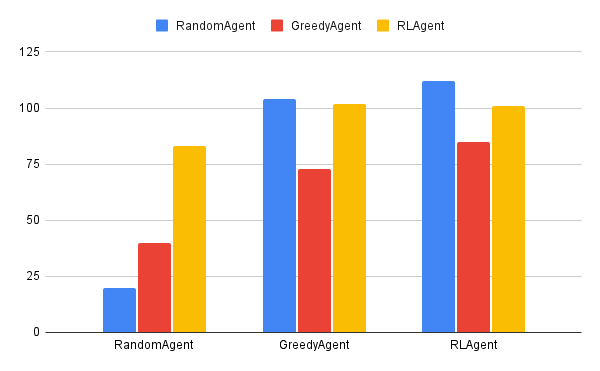
\includegraphics[width=\linewidth]{figures/chart}
	\caption{Experiment results. On the x-axis are the agents (starting players) being evaluated and on the y-axis the average amount of points earned during the experiments.}
	\label{fig:Results}
\end{figure}

The above-mentioned results show that the engine's performance issues heavily
impacted the ability of the agent based on reinforcement learning to learn the game.
Based on this results team decided the next steps should be to improve the engine's
throughput as to increase the learning rate of the agent.


\begin{thebibliography}{00}
\bibitem{CarcassoneRules}
K. Wrede, Carcassonne rules, Z-Man Games, 2016.
% https://images.zmangames.com/filer\_public/d5/20/d5208d61-8583-478b-a06d-b49fc9cd7aaa/zm7810\_carcassonne\_rules.pdf

\bibitem{GolangPipeline}
S. Ajmani, Go Concurrency Patterns: Pipelines and cancellation, The Go Blog, 2014: \url{https://go.dev/blog/pipelines}

\bibitem{AlphaGoAlgorithm}
Silver, D., Schrittwieser, J., Simonyan, K. et al.\ Mastering the game of Go without human knowledge. Nature 550, 354–359 (2017). \url{https://doi.org/10.1038/nature24270}

\bibitem{AlphaGoBlog}
Google DeepMind. AlphaGo. \url{https://deepmind.google/research/breakthroughs/alphago/} (accessed: 28.05.2024)

\bibitem{AlphaGoZeroBlog}
David Silver and Demis Hassabis. Alpha{G}o {Z}ero: {S}tarting from scratch. \url{https://deepmind.google/discover/blog/alphago-zero-starting-from-scratch/} (accessed: 28.05.2024)

\bibitem{AlphaZero}
 Silver, David; Hubert, Thomas; Schrittwieser, Julian; Antonoglou, Ioannis; Lai, Matthew; Guez, Arthur; Lanctot, Marc; Sifre, Laurent; Kumaran, Dharshan; Graepel, Thore; Lillicrap, Timothy; Simonyan, Karen; Hassabis, Demis (December 5, 2017). "Mastering Chess and Shogi by Self-Play with a General Reinforcement Learning Algorithm". arXiv:1712.01815 [cs.AI].

\bibitem{AlphaGoZero}
Silver, D., Schrittwieser, J., Simonyan, K. et al. Mastering the game of Go without human knowledge. Nature 550, 354–359 (2017). \url{https://doi.org/10.1038/nature24270}

\bibitem{MasterThesisCarcassonne}
C. Heyden, Implementing a computer player for Carcassonne, Master's thesis, Department of Knowledge Engineering, Maastricht University, 2009,
pages 13-14.
% https://project.dke.maastrichtuniversity.nl/games/files/msc/MasterThesisCarcassonne.pdf

\bibitem{gopy}
The go-python Authors, gopy project: \url{https://github.com/go-python/gopy}

\bibitem{LanguageBindings}
Wikipedia contributors, Language binding, Wikipedia, The Free Encyclopedia, 2024:
\url{https://en.wikipedia.org/wiki/Language\_binding}
\end{thebibliography}
\end{document}
